\documentclass[12pt]{article}

\usepackage[a4paper, margin=1in]{geometry}
\usepackage{fancyhdr}
\usepackage{titling}
\usepackage[latvian]{babel}
\usepackage{graphicx}
\usepackage{float}
\usepackage{dirtytalk}
\usepackage{gensymb}
\usepackage[utf8]{inputenc}
\usepackage[T1]{fontenc} 
\usepackage{amsmath}
\usepackage{hyperref}

\newlength\tindent
\setlength{\tindent}{\parindent}
\setlength{\parindent}{0pt}
\renewcommand{\indent}{\hspace*{\tindent}}

\fancypagestyle{plain}{
  \fancyhf{}
  \fancyhead[R]{ Andrejs Cvečkovskis \\ ac24005 \\ Kurss \say{Zinātniskā programmēšana fiziķiem}}
  \renewcommand{\headrulewidth}{0pt}
}

\title{\vspace{-1cm}\centering Laboratorijas darbs \\[1ex] \large \say{Statistika} \vspace{-6em}}
\author{}
\date{}  
\begin{document}
\maketitle

1. Kurā pilsētā – Liepājā vai Daugavpilī ir siltāks? Salīdzini gan vidējās, gan mediānas! Pamato savu atbildi!\\

\textbf{Atbilde:} Vidēji siltāks Liepājā; pēc mediānas - Daugavpilī. \\

\textbf{Pamatojums:}

\begin{verbatim}
means   = temperature.mean() 
medians = temperature.median()

warmer_mean   = 'Daugavpilī' if means['Daugavpils'] > 
means['Liepāja'] else 'Liepājā'
warmer_median = 'Daugavpilī' if medians['Daugavpils'] > 
medians['Liepāja'] else 'Liepājā'

print(f"Vidējā temperatūra (°C):\n{means.round(2)}")
print(f"\nMediāna (°C):\n{medians.round(2)}")
print('\nRezultāts:')
print(f"Siltāks **vidēji** ir: {warmer_mean}")
print(f"Siltāks pēc **mediānas** ir: {warmer_median}")
\end{verbatim}

2. Salīdzini ar pandas un numpy iegūtās vērtības savā starpā gan vidējai temperatūrai, gan standartnovirzei! Vai ir kādas atšķirības? Kāpēc? Kura atbilde ir precīzāka? Kāds nosacījums ir jāuzstāda, lai abas atbildes sakristu?\\

\textbf{Atbilde:} Gan ar \texttt{NumPy}, gan ar \texttt{Pandas} iegūtās vidējās temperatūras sakrīt, jo \texttt{Pandas} metodes iekšēji izmanto to pašu \texttt{np.mean} algoritmu. Atšķirība parādās standartnovirzē: \texttt{np.std} pēc noklusējuma izmanto \texttt{ddof=0}, kas atbilst populācijas jeb pilnā datu kopuma standartnovirzei, savukārt \texttt{pd.series.std} pēc noklusējuma izmanto \texttt{ddof=1}, kas ir izlases standartnovirze ar Besela labojumu \cite{Reichmann1961}. Ja temperatūru rindās ir pilns mērījumu kopums un ekstrapolē uz plašāku populāciju, tad statistiski korektāka ir \texttt{NumPy} vērtība. Ja datus uztver kā izlasi no lielākas populācijas, tad nepieciešama \texttt{ddof=1} korekcija, tāpēc \texttt{Pandas} sniegtā vērtība ir piemērotāka. Atšķirība starp abiem rezultātiem samazinās, pieaugot novērojumu skaitam.\\

\textbf{Pamatojums:}
\begin{table}[h]
\centering
\begin{tabular}{lcccc}
\hline
            & mean\_numpy & mean\_pandas & std\_numpy (ddof=0) & std\_pandas (ddof=1) \\
\hline
Daugavpils  & 5.711 & 5.711 & 11.374 & 11.389 \\
Liepāja     & 6.167 & 6.167 &  9.722 &  9.735 \\
\hline
\end{tabular}
\end{table}

\begin{verbatim}
mean_np   = temperature.apply(np.mean)                       
std_np    = temperature.apply(np.std, ddof=0)              

mean_pd   = temperature.mean()                            

std_pd    = temperature.std(ddof=1)                        

compare = pd.DataFrame({
    'mean_numpy' : mean_np,
    'mean_pandas': mean_pd,
    'std_numpy (ddof=0)' : std_np,
    'std_pandas (ddof=1)': std_pd
})

print(compare.round(3))
\end{verbatim}

3. Uzzīmē varbūtību sadalījuma funkciju (\textit{cumulative distribution function}) Daugavpilij. Neaizmirsti par procentiļu atzīmēšanu ar funkciju \texttt{np.percentile}.\\ 

\textbf{Atbilde:}
\begin{center}
    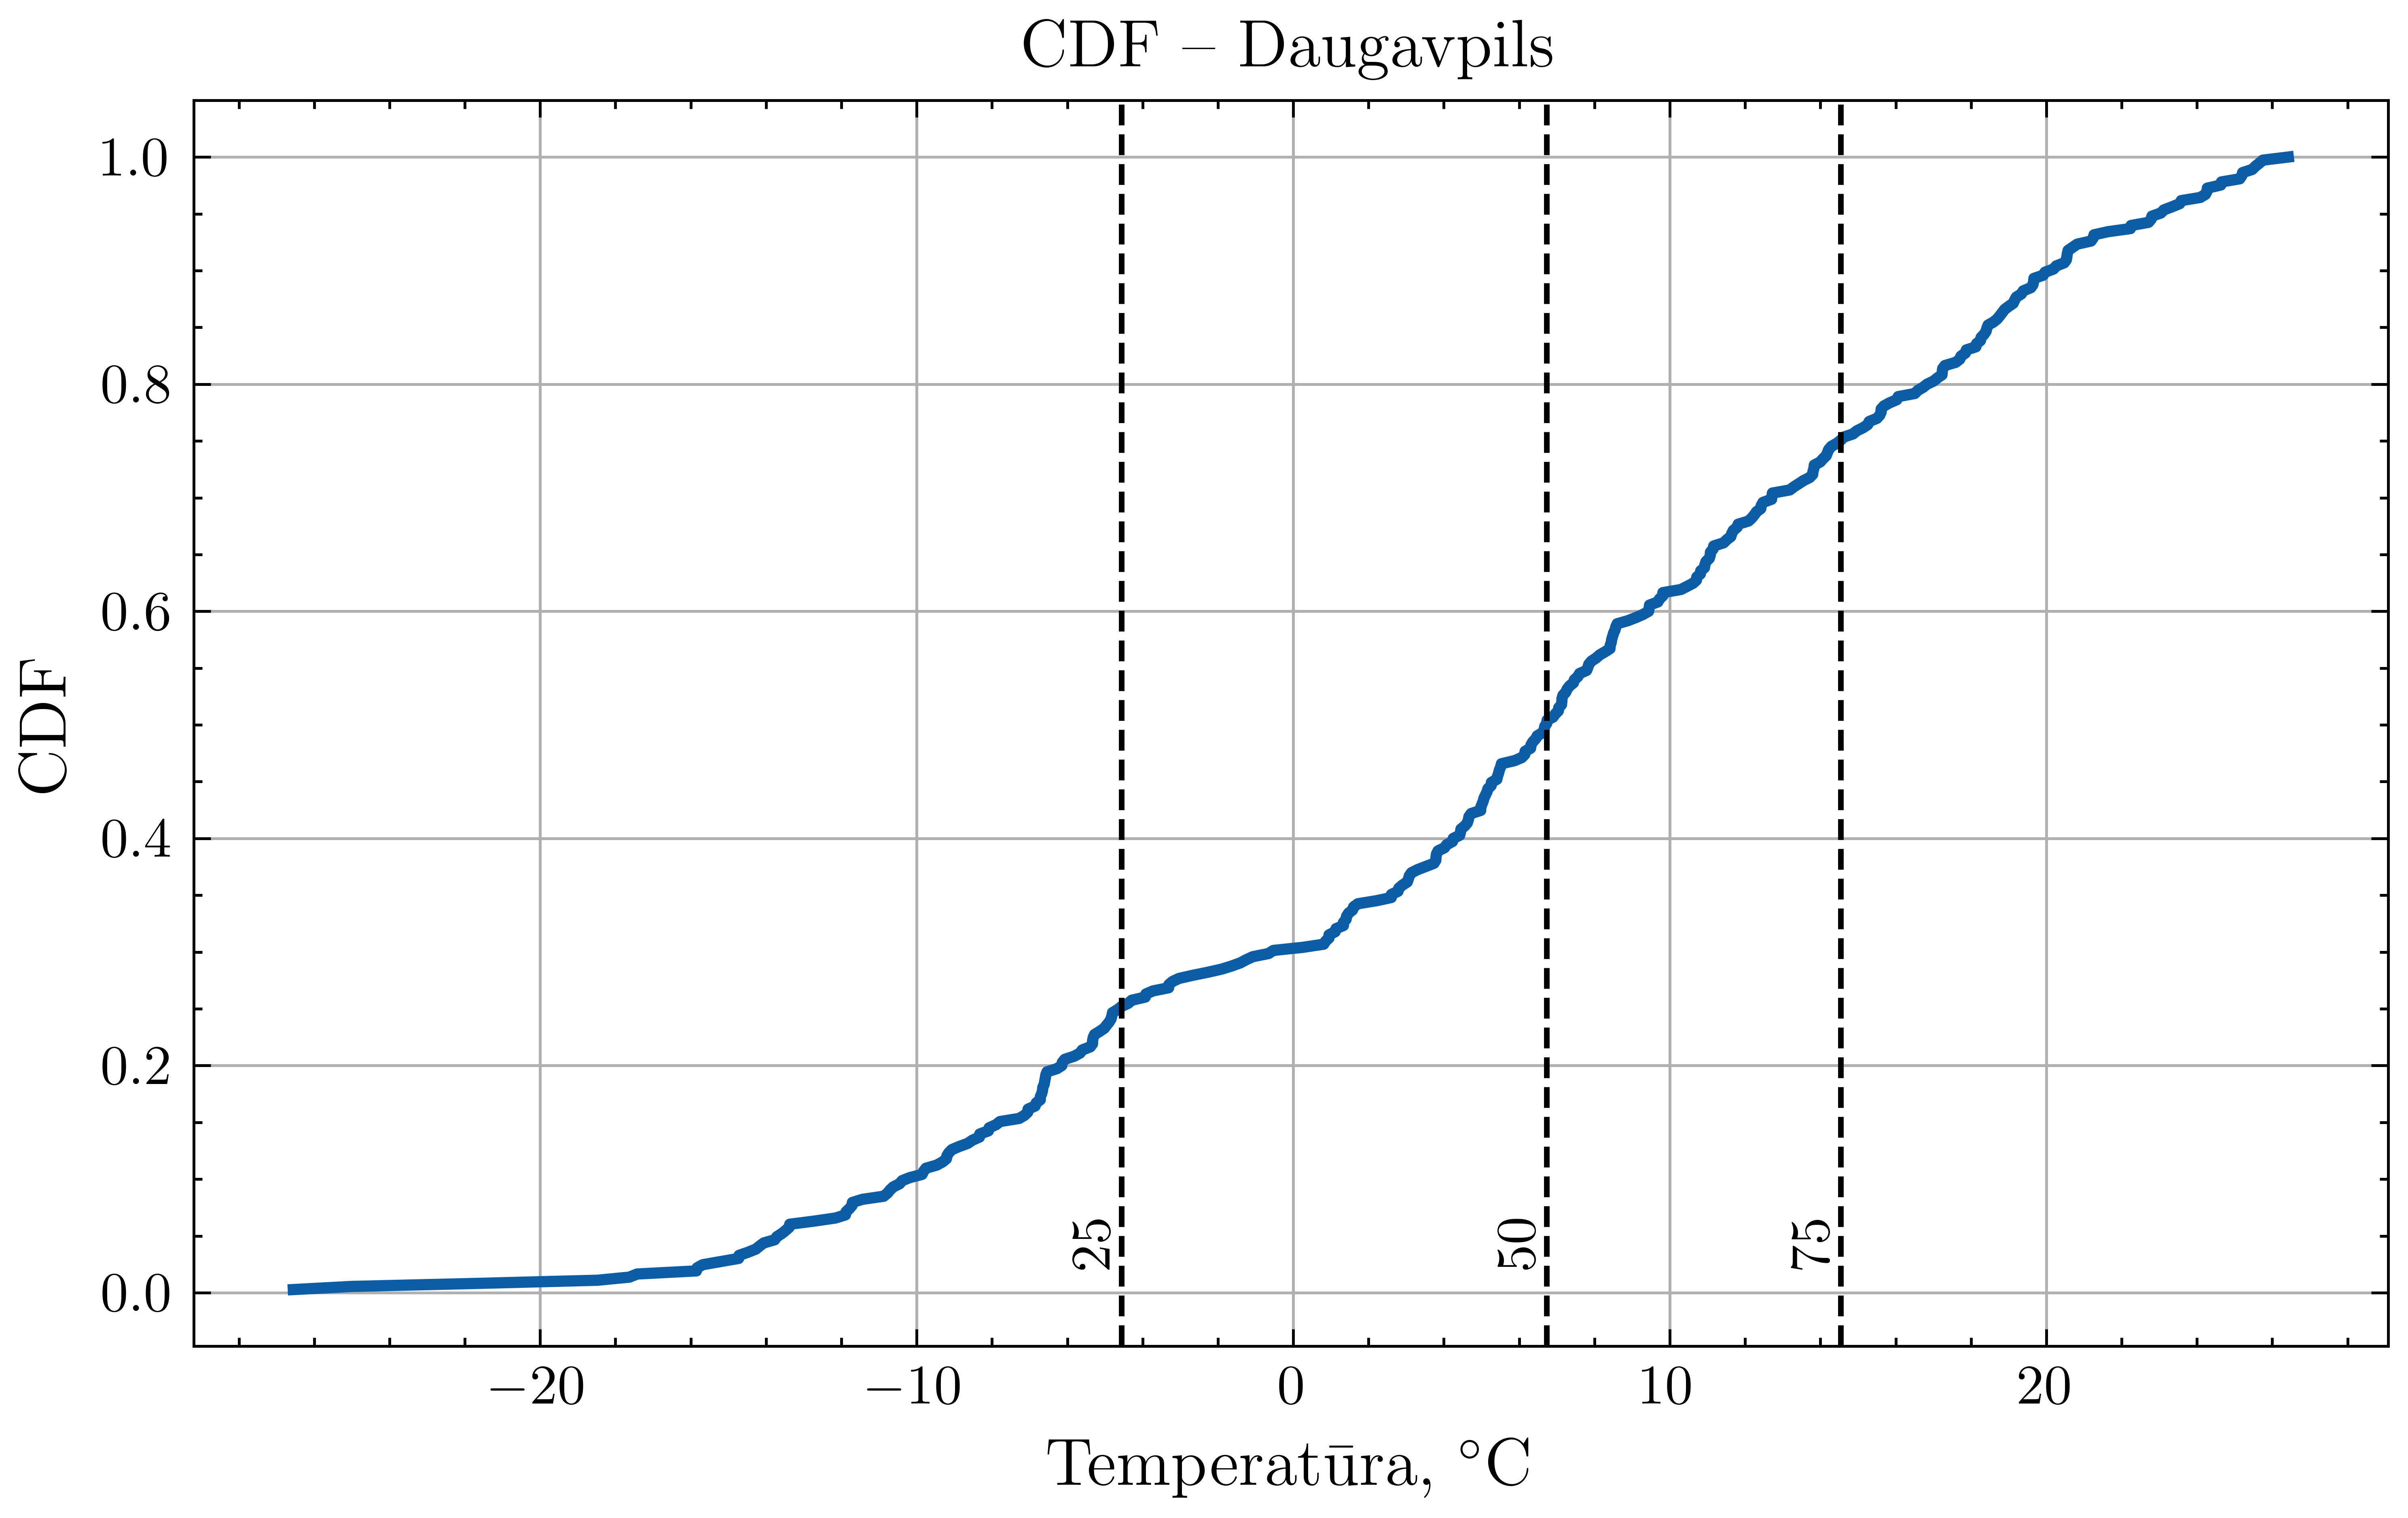
\includegraphics[]{cdf_daugavpils.png}
\end{center}

\textbf{Pamatojums:}
\begin{verbatim}
data = Daug_t["temperature"].dropna().values

sorted_vals = np.sort(data)
cdf = np.arange(1, len(sorted_vals) + 1) / len(sorted_vals)

pcts = [25, 50, 75]
vals = np.percentile(data, pcts)

fig, ax = plt.subplots(figsize=(7, 4))
ax.plot(sorted_vals, cdf, lw=2, label="CDF")

for pct, val in zip(pcts, vals):
    ax.axvline(val, color="k", linestyle="--", linewidth=1)
    ax.text(val, 0.02, rf"{pct} %", rotation=90, va="bottom", ha="right")

ax.set_xlabel("Temperatūra, $^{\circ}$C", fontsize=12)
ax.set_ylabel("CDF", fontsize=12)
ax.set_title("CDF – Daugavpils")
ax.grid(True)
plt.savefig(os.path.join(path, "cdf_daugavpils.png"), dpi=1000)
plt.show()
\end{verbatim}

4. Uzzīmē histogrammas neizmantojot gatavas funkcijas un atzīmē kvartiles.\\

\textbf{Atbilde:}
\begin{center}
    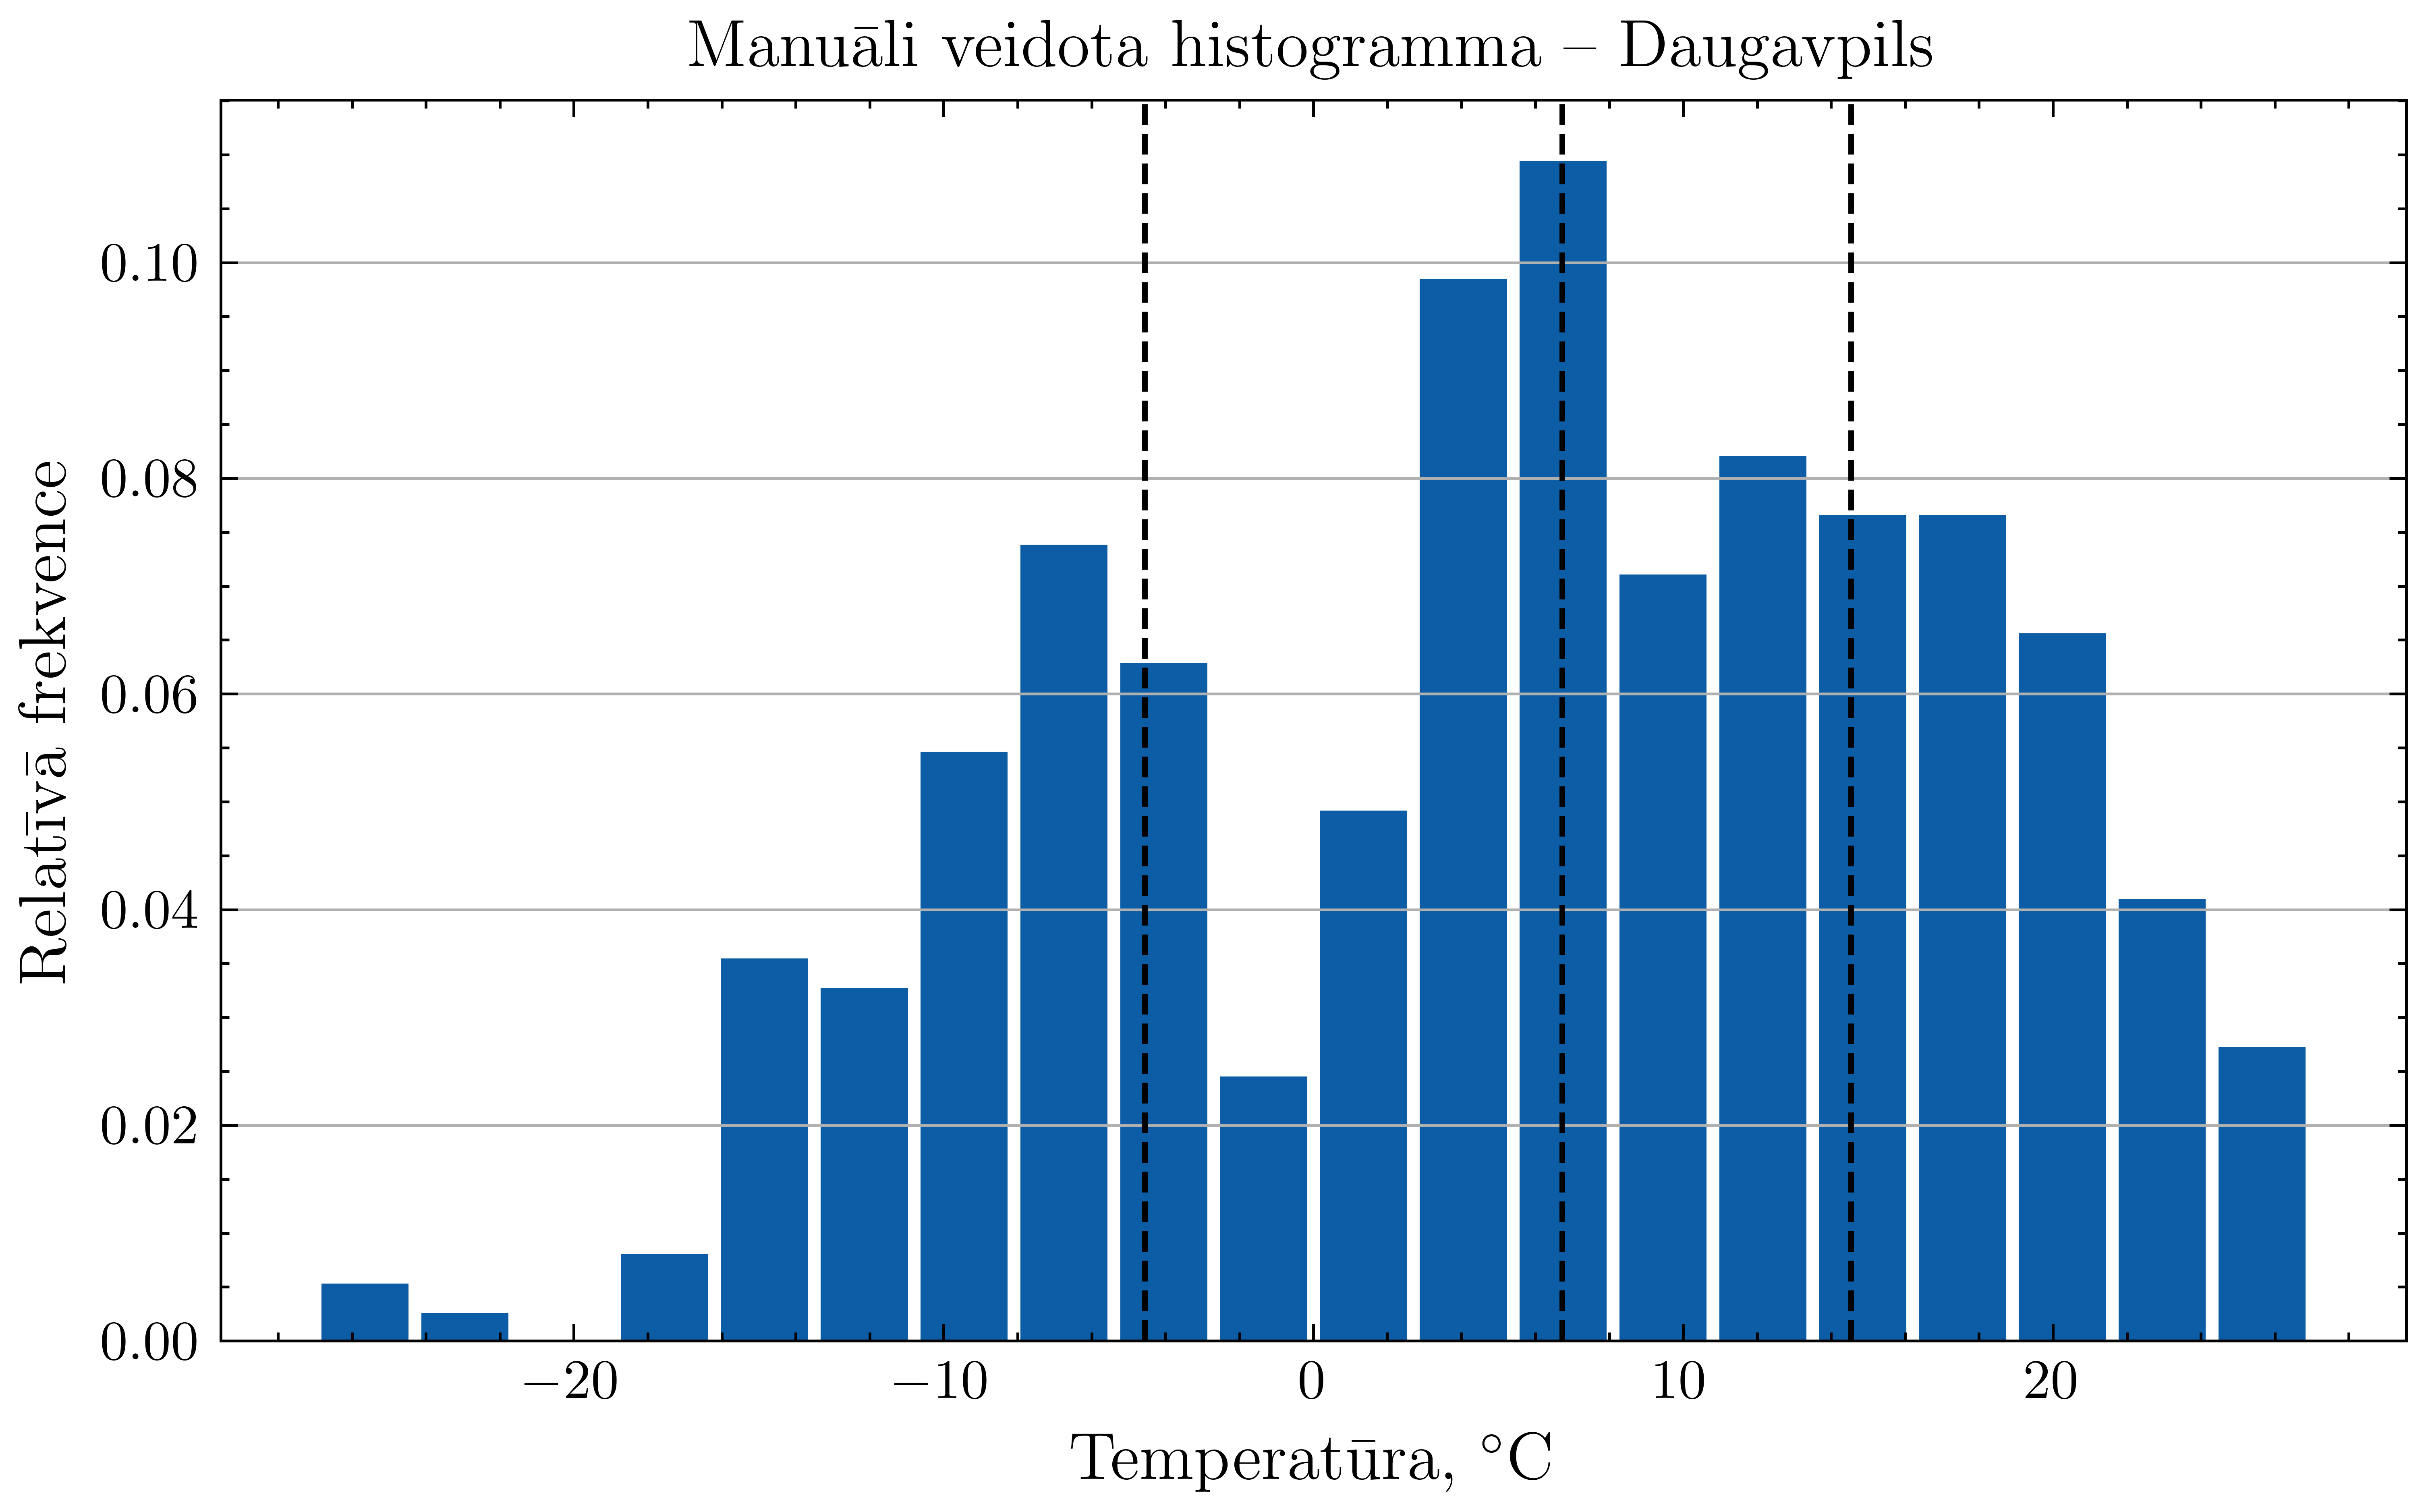
\includegraphics[]{hist_daugavpils.png}
\end{center}\\

\textbf{Pamatojums:}
\begin{verbatim}
data = Daug_t["temperature"].dropna().values
bins = 20
xmin, xmax = -27, 27
bin_edges = np.linspace(xmin, xmax, bins + 1)
counts = np.zeros(bins, dtype=int)

for v in data:
    if xmin <= v < xmax:
        idx = int((v - xmin) / (xmax - xmin) * bins)
        counts[idx] += 1
    elif v == xmax:      # robežvērtība iet pēdējā binā
        counts[-1] += 1

fig, ax = plt.subplots(figsize=(7, 4))
bin_centers = (bin_edges[:-1] + bin_edges[1:]) / 2
width = bin_edges[1] - bin_edges[0]
ax.bar(bin_centers, counts / counts.sum(), width=width * 0.9,
       align="center", edgecolor="white", linewidth=0.5)

q25, q50, q75 = np.percentile(data, [25, 50, 75])
for q in [q25, q50, q75]:
    ax.axvline(q, color="k", linestyle="--", linewidth=1)

ax.set_xlabel("Temperatūra, $^{\circ}$C", fontsize=12)
ax.set_ylabel("Relatīvā frekvence", fontsize=12)
ax.set_title("Manuāli veidota histogramma – Daugavpils")
ax.grid(axis="y")
plt.savefig(os.path.join(path, "hist_daugavpils.png"), dpi=1000)
plt.show()
\end{verbatim}

5. Boxplot ir attēloti sadalījumu raksturojošie lielumi: mediāna, 25 un 75 perc, utt. Aprēķini to skaitliskās vērtības!\\

\textbf{Atbilde:}
\begin{table}[h]
\centering
\begin{tabular}{lrrrrrr}
\hline
Pilsēta & Median & Q\textsubscript{1} & Q\textsubscript{3} & IQR & Whisker\(_\text{low}\) & Whisker\(_\text{high}\) \\
\hline
Daugavpils & 6.73 & -4.56 & 14.54 & 19.10 & -33.21 & 43.19 \\
Liepāja    & 6.31 & -1.44 & 13.65 & 15.09 & -24.07 & 36.28 \\
\hline
\end{tabular}
\end{table}\\

\textbf{Pamatojums:}
\begin{verbatim}
# Raksti savu atbildi šeit:
stats = temperature.agg(
    median  = ("Daugavpils", "median"),
).T  # sākam ar tukšu karkasu, lai vēlāk pievienotu abas pilsētas

for col in temperature.columns:
    q1, q3 = temperature[col].quantile([0.25, 0.75])
    med    = temperature[col].median()
    iqr    = q3 - q1
    whisk_low  = q1 - 1.5 * iqr
    whisk_high = q3 + 1.5 * iqr
    stats.loc[col, ["median", "q1", "q3", "iqr", "whisker_low", "whisker_high"]] = [
        med, q1, q3, iqr, whisk_low, whisk_high
    ]

print(stats.round(2))
\end{verbatim}

6. Atceries jautājumu \texttt{notebook} sākumā par to, kura pilsēta ir vidēji siltāka. Aplūko Daugavpils un Liepājas sadalījumu formu – kādas īpatnības ir iespējams ieraudzīt?\\ 

\textbf{Atbilde:} Daugavpils sadalījums ir izteikti bimodāls, ar diviem skaidriem maksimumiem – viens ap aukstām ziemas temperatūrām un otrs ap siltām vasaras temperatūrām. Tas liecina par lielāku temperatūru amplitūdu un kontinentālāku klimatu. Savukārt Liepājas sadalījums ir simetriskāks un koncentrētāks ap centrālajām vērtībām, kas norāda uz mērenāku un stabilāku klimatu, iespējams, jūras ietekmes dēļ.

Salīdzinot vidējo un mediānu, vidējā temperatūra ir augstāka Liepājā, kas nozīmē, ka kopumā gada griezumā tā ir siltāka. Mediāna savukārt ir augstāka Daugavpilī, kas nozīmē, ka vairāk nekā puse no dienām bija siltākas nekā Liepājā.\\

7. Pie kāda \texttt{n} ģenerētie skaitļi labi atbilst vienmērīgam sadalījumam?\\ 

\textbf{Atbilde:} Histogrammas skaidri parāda, ka pie $n=3 $ jeb 1000 skaitļiem sadalījums sāk līdzināties vienmērīgam – joslas kļūst līdzīga augstuma un aptver visu intervālu no 0 līdz 1 bez izteiktiem tukšumiem vai pīķiem. Pie $n=4$ un vairāk šī līdzība kļūst vēl izteiktāka. Līdz ar to, var secināt, ka vienmērīgam sadalījumam atbilst ģenerēto skaitļu skaits no aptuveni $10^3$ un uz augšu.
\begin{center}
    \includegraphics[width=1\linewidth]{uniform_histograms.png}
\end{center}\\

\textbf{Pamatojums:}
\begin{verbatim}
fig, axs = plt.subplots(2, 3, figsize=(18, 10))
axs = axs.flatten()

for i, n in enumerate(range(1, 7)):
    x = np.random.rand(10**n)
    axs[i].hist(x, bins=10, range=(0, 1), density=True, 
    edgecolor='white', linewidth=0.5)
    axs[i].set_title(f"$10^{n}$", fontsize=24)
    axs[i].grid(axis='y')
    axs[i].set_ylim(0, 1.5)

plt.suptitle("Vienmērīgi sadalītu skaitļu histogrammas dažādiem $n$", fontsize=26)
plt.tight_layout(rect=[0, 0, 1, 0.96])
plt.savefig(os.path.join(path, "uniform_histograms.png"), dpi=1000)
plt.show()
\end{verbatim}\\

8. Iedomāsimies, ka šī problēma tiek apskatīta laboratorijas darbā. Ko laboratorijas darbos izmantotā kļūdu teorija saka par jaudas relatīvās kļūdas atkarību no diametra kļūdas (netiešā mērīšana)? Salīdzini laboratorijas darbos iegūtos aprēķinus ar to, ko var redzēt histogrammās!\\

\textbf{Atbilde:}
Eksperimentā tiek mērīts stieples diametrs $d$, kurš tiek uzskatīts par gadījuma lielumu ar normālu sadalījumu. No šī diametra tiek aprēķināta jauda, kas izdalās stieplē, ja tai cauri plūst zināma strāva $I$. Pieņemot, ka konstantes $I$, $\rho$, $L$ ir zināmas ar nenozīmīgu kļūdu un ka
\[
P = \frac{4 I^2 \rho L}{\pi d^2} \quad \Rightarrow \quad P = \frac{1}{d^2},
\]
tad var izmantot kļūdu formulu netiešai mērīšanai:
\[
\frac{\Delta P}{P} = \left| \frac{dP}{dd} \cdot \frac{d}{P} \right| \cdot \frac{\Delta d}{d} = 2 \cdot \frac{\Delta d}{d}.
\]

Tika simulēti $n = 10000$ diametra mērījumi ar normālu sadalījumu:
\[
\bar{d} = 0{,}9996, \quad \sigma_d = 0{,}0492, \quad \text{SEM}_d = \frac{\sigma_d}{\sqrt{n}} = 0{,}00049,
\]
\[
\Rightarrow \text{relatīvā kļūda vidējai vērtībai: } r_{\bar{d}} = \frac{\text{SEM}_d}{\bar{d}} = 0{,}000492 \quad (0{,}0492\%).
\]

No šiem datiem tika aprēķināta jauda:
\[
\bar{P} = 1{,}0082, \quad \sigma_P = 0{,}1003, \quad \text{SEM}_P = \frac{\sigma_P}{\sqrt{n}} = 0{,}001003,
\]
\[
\Rightarrow r_{\bar{P}} = \frac{\text{SEM}_P}{\bar{P}} = 0{,}000995 \quad (0{,}0995\%).
\]

Teorētiskā prognoze relatīvajai jaudas kļūdai:
\[
r_{\bar{P}, \text{prognozēts}} = 2 \cdot r_{\bar{d}} = 2 \cdot 0{,}000492 = 0{,}000985.
\]

Reāli aprēķinātā kļūda:
\[
r_{\bar{P}, \text{aprēķināts}} = 0{,}000995.
\]

Attiecība starp aprēķināto un teorētisko kļūdu:
\[
\frac{r_{\bar{P}}}{r_{\bar{d}}} \approx 2{,}02.
\]

Tā kā jauda $P$ ir atkarīga no diametra $d$ kvadrāta apgrieztās vērtības, tad neliela kļūda diametrā noved pie divreiz lielākas kļūdas aprēķinātajā jaudā. Gan teorētiskā prognoze, gan aprēķini to apstiprina ar augstu precizitāti.

To vēl papildus var novērot histogrammās: diametra histogramma ir simetriska un šaura, kas raksturīgs normālam sadalījumam ar mazu izkliedi. Savukārt jaudas histogramma ir platāka un asimetriska pa labi, kas atspoguļo to, kā nelineāra atkarība (piemēram, $1/d^2$) pastiprina novirzes un kļūdas. Tādējādi arī grafiski redzams, ka jauda ir daudz jutīgāka pret izmaiņām diametrā, kā to paredz kļūdu pārmantošanas aprēķini.\\

9. Attēlo Stjūdenta sadalījumu ({\href{https://en.wikipedia.org/wiki/Student%27s_t-distribution}{Links}) dažādām brīvības pakāpes vērtībām $\nu$ (gan \texttt{pdf}, gan \texttt{cdf}; \texttt{cdf} aprēķina izmantojot integrēšanu). Parādi īpašgadījumu, kad Stjūdenta sadalījums pārvēršas par normālo jeb Gausa sadalījumu. Salīdzini ar teorētisko Gausa sadalījuma līkni (gan \texttt{pdf}, gan \texttt{cdf}). Šim uzdevumam obligāti pievieno kodu.\\

\textbf{Atbilde:}

\emph{PDF.}  
Stjūdenta $t$-sadalījumam ir biezākas “astes’’ nekā normālajam
sadalījumam, tādēļ pie maziem $|x|$ tā blīvums ir \emph{zemāks},
bet pie lieliem $|x|$ – \emph{augstāks} par Gausa blīvumu.
Piemēram pie $x=1$:
\[
\frac{f_{t}(1;\nu)}{f_{N}(1)}=
\begin{cases}
0.66 & (\nu=1),\\
0.80 & (\nu=2),\\
0.91 & (\nu=5),\\
0.98 & (\nu=30),\\
1.00 & (\nu=100).
\end{cases}
\]
Savukārt pie $x=2$ attiecība jau kļūst $>1$, piem.\ $1.26$ ($\nu=2$),
kas ilustrē garākās astes.

Kad $\nu\!\to\!\infty$ (praktiski jau pie $\nu\gtrsim30$)
$t$-PDF gandrīz sakrīt ar Gausa PDF: maksimuma augstums  
$f_{t}(0;\,30)\approx0.396$ pret $f_{N}(0)=1/\sqrt{2\pi}\approx0.399$  
atšķiras mazāk nekā par $1\%$.

\emph{CDF.}  
Kumulatīvā funkcija rāda to pašu tendenci.
Pie pozitīviem $x$ $t$-CDF aug \emph{lēnāk} (lielāka masa astēs),
tāpēc starpība $F_{t}(x;\nu)-F_{N}(x)$ ir negatīva:
\[
F_{t}(1;\nu)-F_{N}(1)=
\begin{cases}
-0.091 & (\nu=1),\\
-0.053 & (\nu=2),\\
-0.014 & (\nu=5),\\
-0.004 & (\nu=30),\\
-0.001 & (\nu=100).
\end{cases}
\]
Pie $\nu=100$ absolūtā atšķirība visā intervālā $x\in[-5,5]$
nepārsniedz $1.4\times10^{-3}$, tādēļ grafikā $t$-CDF un Gausa CDF
praktiski pārklājas.

\emph{Secinājums.}  
Mazām brīvības pakāpēm $t$-sadalījumam ir izteikti biezas astes
(un dispersija ir bezgalīga, ja $\nu\le 2$),
bet, pieaugot $\nu$, gan PDF, gan CDF gludi konverģē
uz normālo sadalījumu; vizuāli būtiskas atšķirības vairs
neredz jau pie $\nu\approx30$.
\\

\begin{center}
    \includegraphics[width=1\linewidth]{student_t_pdf.png}
\end{center}

\begin{center}
    \includegraphics[width=1\linewidth]{student_t_cdf.png}
\end{center}
\textbf{Pamatojums:}
\begin{verbatim}
x = np.linspace(-5, 5, 500)

# degrees of freedom to display # can anyone truly be free?
dfs = [1, 2, 5, 10, 30, 100]

plt.figure(figsize=(10, 6))
for df in dfs:
    plt.plot(x, scipy.stats.t.pdf(x, df), label=rf"$\nu={df}$")
plt.plot(x, scipy.stats.norm.pdf(x), "k--", lw=1.8, label="Gausa sadalījums")
plt.title("Stjūdenta $t$-sadalījums (PDF) dažādām brīvības pakāpēm", fontsize=20)
plt.xlabel(r"$x$", fontsize=18)
plt.ylabel("Blīvums", fontsize=18)
plt.grid(alpha=0.3)
plt.legend()
plt.tight_layout()
plt.savefig(os.path.join(path, "student_t_pdf.png"), dpi=1000)
plt.show()

plt.figure(figsize=(10, 6))

for df in dfs:
    pdf_vals = scipy.stats.t.pdf(x, df)          # PDF samples
    cdf_vals = cumulative_trapezoid(pdf_vals, x, initial=0)  # trapezoidal integral
    # normalise (tails outside the grid give a tiny deficit)
    cdf_vals /= cdf_vals[-1]
    plt.plot(x, cdf_vals, label=rf"$\nu={df}$")

# Gaussian reference (analytic CDF is fine)
plt.plot(x, scipy.stzats.norm.cdf(x),
         "k--", lw=1.8, label="Gausa sadalījums")

plt.title("Stjūdenta $t$-sadalījums (CDF) — integrējot PDF", fontsize=20)
plt.xlabel(r"$x$", fontsize=18)
plt.ylabel("Kumulatīvā varbūtība", fontsize=18)
plt.grid(alpha=0.3)
plt.legend()
plt.tight_layout()
plt.savefig(os.path.join(path, "student_t_cdf.png"), dpi=1000)
plt.show()
\end{verbatim}

\newpage

\renewcommand{\refname}{Izmantotā literatūra}
\bibliographystyle{plain}
\bibliography{bib}

\end{document}